\documentclass[11pt,a4paper]{ivoa}
\input tthdefs
\input gitmeta

\customcss{custom.css}

\usepackage{xifthen}
\lstloadlanguages{XML,SQL}
\lstset{flexiblecolumns=true,basicstyle=\ttfamily}
 
\iftth
\newenvironment{args}%
{\begin{html}<ul>\end{html}\def\arg##1(##2){\begin{html}<li><i>\end{html}%
  ##1 \begin{html}</i>(<code>\end{html}##2\begin{html}) </code>\end{html}}}%
{\begin{html}</ul>\end{html}}

\newenvironment{examples}%
{\begin{html}<p><strong>Examples</strong></p><ul>\end{html}%
  \def\example{\begin{html}<li><code>\end{html}}%
  \def\becomes{\begin{html}</code><br/>\end{html} returns
    \begin{html}<code>\end{html}}%
  \def\done##1.{\begin{html}</code> <span class="explanation">\end{html}
    ##1
    \begin{html}</span></li>\end{html}}}%
{\begin{html}</ul>\end{html}}

\else
% definition pulled out of doc to hide it from tth (which gets confused
% by ifthenelse

\newenvironment{args}%
% this is *only* for use within a description environment
  {\hfil % let definition label stand on a line of its own.
    \def\arg##1(##2){\item {\textit{##1} (\texttt{##2})}}
    \begin{list}{$\bullet$}{\topsep=0pt\partopsep=0pt\parsep=0pt}
    }%
  {\end{list}}

\newenvironment{examples}%
  {\par\bigbreak
    \noindent\textbf{Examples} (non-normative)\nobreak\par
    \nobreak\vskip 3pt plus 1pt
    \def\example{\par\noindent}%
    \def\becomes{\ifhmode\hfil\break\fi\strut\qquad$\to$ }%
    \def\done##1.{\ifthenelse{\isempty{##1}}{\par}{%
        \hfil\break{\footnotesize\fontshape{it}\selectfont
        ##1.\par}}\vskip 4pt plus 2pt}}%
  {\relax}



\fi


\title{Catalogue of ADQL User Defined Functions}

% see ivoatexDoc for what group names to use here
\ivoagroup{DAL}

\author[https://wiki.ivoa.net/twiki/bin/view/IVOA/JonJuaristiCampillo]{Jon Juaristi Campillo}
\author[https://wiki.ivoa.net/twiki/bin/view/IVOA/MarkusDemleitner]{Markus Demleitner}


\editor[https://wiki.ivoa.net/twiki/bin/view/IVOA/JonJuaristiCampillo]{Jon Juaristi Campillo}

\previousversion[http://ivoa.net/documents/udf-catalogue/20190925]{PEN-20190925}
       

\begin{document}
\begin{abstract}
The IVOA Astronomical Data Query Language (ADQL) has the extension
facility of user defined functions (UDFs).  While service operators are
free to define these as they see fit, it is clearly advantageous if
identical functionality is available under identical names in different
services.  Therefore, ADQL 2.1 has introduced the \verb|ivo_| prefix,
reserved for functions with agreed-upon semantics.  This endorsed note
contains this agreement and, via its updates, is the means of updating
it.  A non-normative appendix lists UDFs declared by registered TAP
services; some of these might be developed into consensus UDFs in later
releases.
\end{abstract}


\section*{Conformance-related definitions}

The words ``MUST'', ``SHALL'', ``SHOULD'', ``MAY'', ``RECOMMENDED'', and
``OPTIONAL'' (in upper or lower case) used in this document are to be
interpreted as described in IETF standard RFC2119 \citep{std:RFC2119}.

The \emph{Virtual Observatory (VO)} is a
general term for a collection of federated resources that can be used
to conduct astronomical research, education, and outreach.
The \href{http://www.ivoa.net}{International
Virtual Observatory Alliance (IVOA)} is a global
collaboration of separately funded projects to develop standards and
infrastructure that enable VO applications.


\section{Introduction}

The Astronomical Data Query Language (ADQL) \citep{2008ivoa.spec.1030O}
has the notion of user defined functions (UDF).  These provide a
light-weight extension mechanism for operators of TAP services.  
For instance, \citet{2016arXiv161109190T} show how they enable the
construction of HEALPix maps although ADQL~2.0 itself entirely lacks
facilities to deal with them.

In order to avoid different signatures or semantics on functions
offering identical or similar functionality,  this document defines UDFs
with names prefixed with \verb|ivo_|.  If services have functions with
this names, they must work as defined here.

In version 1.0, this note documents a consensus 
on such functions where it has been
reached within other standards or in the review of this document.  

In the future, where UDFs are not naturally associated with a
particular standard, they can be proposed by editing this document and
starting the Endorsed Note process \citep{2017ivoa.spec.0517G} on the
changes.  In effect, this endorsed note is the management tool for
the \verb|ivo_| ``namespace'' in ADQL user defined functions.

Note that no function given here is required to be present in a generic
TAP service (though other standards may pose such requirements;
\verb|ivo_hashlist_has|, for instance, is required by both
RegTAP and EPN-TAP).  However, if a service implements any UDF with a
name mentioned in this document, its semantics must be as specified here.

Informationally, in each revision of this document, we also run an
all-VO survey of user defined functions in registered TAP services.  A
digest of this survey is given in the non-normative
Appendix~\ref{app:otherudfs}.

\subsection{Role within the VO Architecture}

\begin{figure}
\centering

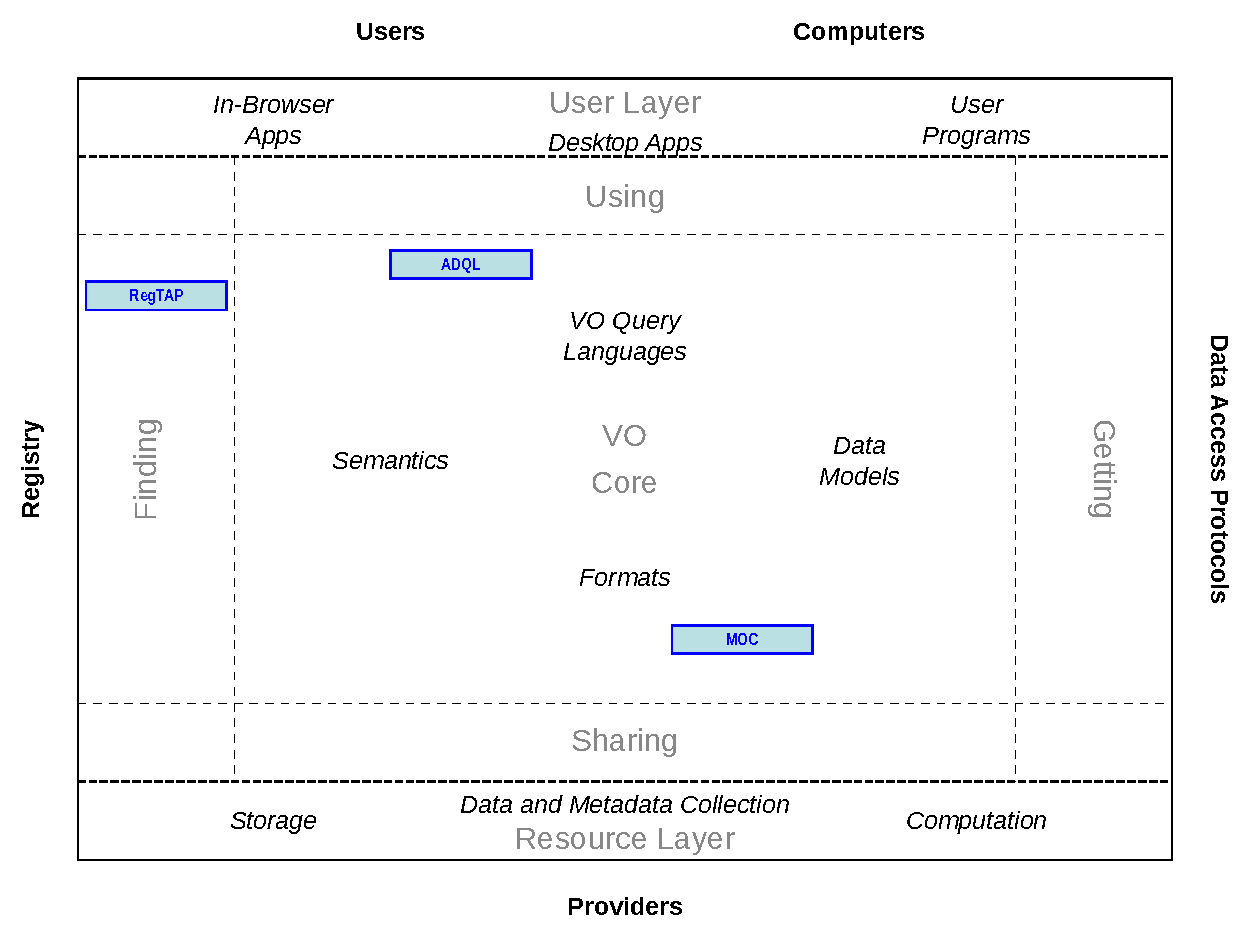
\includegraphics[width=0.9\textwidth]{role_diagram.pdf}
\caption{Architecture diagram for the UDF catalogue.}
\label{fig:archdiag}
\end{figure}

Fig.~\ref{fig:archdiag} shows the role this document plays within the
IVOA architecture \citep{note:VOARCH}.  It relates to the following
other standards:

\begin{bigdescription}
\item[ADQL \citep{2008ivoa.spec.1030O}] This endorsed note defines the
user defined functions with the \verb|ivo_| prefix.  While ADQL 2.0
does not treat those as special, they can be (and have been) used there
already.  Normative language on \verb|ivo_| is expected to become
part of ADQL 2.1.

\item[RegTAP \citep{2019ivoa.spec.1011D}] RegTAP first defined some of the
UDFs defined here.  It is expected that later versions of RegTAP will
refer to this note rather than maintaining a second definition, and
deferring the actual definition of UDFs to this note should be the
standard way of introducing UDFs used or required by a standard in the future.

\item[MOC \citep{2019ivoa.spec.1007F}] The HEALPix functions defined
here build on terminology introduced in the MOC specification.
\end{bigdescription}


\section{List of IVOA user defined functions}

The functions are defined through a brief human-readable description of
what the function does, followed by a closer discussion of the
parameters, the return value, and the authority the UDF was drawn from.

In the parameter definitions, we do not distinguish between different
precisions of floating point arguments.  Where we write \texttt{REAL}, the
expectation is that the functions accept floating point values of any
precision.  Similarly, we write \texttt{TEXT} for anything sufficiently
string-like, be it \texttt{CHAR(n)}, \texttt{VARCHAR(*)}, or something
comparable.

Most functions are accompanied by examples, which are intended to make
the the effects of the functions clearer and give implementors a
starting point for tests.  Where examples disagree with the
specification text, the text is normative.

While ADQL does not support standalone evaluation of functions, a query
like 
\begin{lstlisting}[language=SQL]
  SELECT TOP 1 <example> AS res FROM TAP_SCHEMA.tables
\end{lstlisting}
will return one row with the function result for simple, non-aggregate
functions.


\subsection{HEALPix-related}

In this section, order and npix are used as in the Multi-Order
Coverage map (MOC) recommendation
\citep{2014ivoa.spec.0602F}.

\subsubsection{ivo\_healpix\_index(hpxOrder, long, lat)}

Returns the index (npix) of the HEALPix cell containing the spherical
point given by longitude \texttt{long} (typically, right ascension) and
latitude \texttt{lat} (typically, declination) at order
\texttt{hpxOrder} in NESTED numbering.

\begin{description}
\item[Parameters]
\begin{args}
	\arg hpxOrder (INTEGER) -- the HEALPix order to use.
	\arg long (REAL) -- longitude of the spherical point to compute the
	index for, in degrees.
	\arg lat (REAL) -- latitude of the spherical point to compute the
	index for, in degrees.
\end{args}

\item[Return type] \texttt{BIGINT}

\item[Source] This document.
\end{description}

\begin{examples}
\example \verb|ivo_healpix_index(0, 1, 1)|
\becomes \verb|4|
\done.

\example \verb|ivo_healpix_index(17, 1, 1)|
\becomes \verb|81609757711|
\done.

\example \verb|ivo_healpix_index(17, 359, -1)|
\becomes \verb|73009064944|
\done.
\end{examples}

\subsubsection{ivo\_healpix\_index(hpxOrder, point)}

Returns the index (npix) of the HEALPix cell containing the spherical
point given by \texttt{point} at order \texttt{hpxOrder} in NESTED
numbering.

\begin{description}
\item[Parameters]
\begin{args}
	\arg hpxOrder (INTEGER) -- the HEALPix order to use.
	\arg point (POINT) -- the position to compute the index for.
\end{args}

\item[Return type] \texttt{BIGINT}

\item[Source] This document.
\end{description}

\begin{examples}
\example \verb|ivo_healpix_index(0, POINT(1, 1))|
\becomes \verb|4|
\done.

\example \verb|ivo_healpix_index(17, POINT('ICRS', 1, 1))|
\becomes \verb|81609757711|
\done.

\example \verb|ivo_healpix_index(17, CENTROID(CIRCLE(359, -1, 3)))|
\becomes \verb|73009064944|
\done.
\end{examples}


\subsubsection{ivo\_healpix\_center(hpxOrder, hpxIndex)}

Returns a POINT corresponding to the center of the HEALPix cell
with index (npix) \texttt{hpxIndex} at order \texttt{hpxOrder} in NESTED
numbering.

\begin{description}
\item[Parameters]
\begin{args}
	\arg hpxOrder (INTEGER) -- the HEALPix order to use.
	\arg hpxIndex (INTEGER) -- the index for which to return the center
	position.
\end{args}


\item[Return type] \texttt{POINT}

\item[Source] This document.
\end{description}

\begin{examples}
\example \verb|ivo_healpix_center(0, 6)|
\becomes \verb|[180., 0.]|
\done as a 2-array with \xmlel{xtype}=\emph{point}.

\example \verb|ivo_healpix_center(17, ivo_healpix_index(17, 23.4, 56.7))|
\becomes \verb|[23.399843462947466, 56.70016214363192]|
\done.

\example \verb|ivo_healpix_center(17, 23.2)|
\becomes undefined
\done Implementations are advised to fail when floating point numbers
are passed as indices, but may choose to do some rounding.
\end{examples}


\subsection{Text-Related}

\subsubsection{ivo\_string\_agg(expression, delimiter)}

An aggregate function returning all values of \texttt{expression} 
concatenated with \texttt{delimiter}.

\begin{description}
\item[Parameters]

\begin{args}
	\arg expression (TEXT) -- a SQL expression giving the strings to
	concatenate.  The expression may be NULL, in which case the row does
	not leave a trace in the result string.
	\arg delimiter (TEXT) -- a string used to concatenate the values of
	\texttt{expression} in each group.
\end{args}

\item[Return type] \texttt{TEXT}

\item[Source] RegTAP \citep{2014ivoa.spec.1208D}
\end{description}

\begin{examples}
\example \begin{lstlisting}[language=SQL]
SELECT ivo_string_agg(table_name, ' <//> ')|
FROM TAP_SCHEMA.tables
WHERE table_name ILIKE 'tap_schema.%'
\end{lstlisting}
\becomes \verb|'tap_schema.columns <//> tap_schema.schemas <//> ta...'|
\done Of course, the actual value depends on the contents of the TAP
schema on the service used to run the query.
\end{examples}

\subsubsection{ivo\_nocasematch(value, pattern)}

Evaluates \texttt{value ILIKE <pattern>} pattern, i.e.,
pattern is defined as for the SQL LIKE operator, but the match is
performed case-insensitively.  Returns
1 if the pattern matches, 0 otherwise.

Databases processing non-ASCII should perform case folding according to
algorithm R2 in section 3.13, ``Default Case Algorithms'' of the Unicode
Standard \citep{std:UNICODE}.

Please note that in ADQL versions higher than ADQL 2.1, the ILIKE
operator should be used instead.

\begin{description}
\item[Parameters]

\begin{args}
	\arg value (TEXT) -- a string-valued SQL expression.
	\arg pattern (TEXT) -- a SQL pattern for LIKE evaluation (i.e.,
	underscore is any character, percent zero or more arbitrary
	characters).
\end{args}

\item[Return type] \texttt{INTEGER}

\item[Source] RegTAP \citep{2014ivoa.spec.1208D}
\end{description}

\begin{examples}
\example\verb|ivo_nocasematch('abcabc', 'ab%')|
\becomes 1
\done.

\example\verb|ivo_nocasematch('ABcabc', 'ab__bc')|
\becomes 1
\done.

\example\verb|ivo_nocasematch('abcabc', '%BC')|
\becomes 1
\done.

\example\verb|ivo_nocasematch('abcabc', 'ABCABC')|
\becomes 1
\done.

\example\verb|ivo_nocasematch('abcabc', 'abcab')|
\becomes 0
\done.
\end{examples}


\subsubsection{ivo\_hasword(haystack, needle)}

Returns 1 if all tokens from the string \texttt{needle} are contained
(in some sense) in the string \texttt{haystack}, 0 otherwise.  This is
intended to support somewhat ``Google-like'', soft string matches.  This
specification does not precisely specify what ``token'' exactly means
and whether stemming or any other normalisation should be performed,
except that matching must be case-insensitive within ASCII, and that
the minimal token definition is a continuous run of ASCII characters.
Implementors are encouraged to attempt a reasonable approximation to
what Web search engines do.

\begin{description}
\item[Parameters]

\begin{args}
	\arg needle (TEXT) -- a string to locate in \texttt{haystack}.
	\arg haystack (TEXT) -- text to match \texttt{needle} in.
\end{args}

\item[Return type] \texttt{INTEGER.}

\item[Source] RegTAP \citep{2014ivoa.spec.1208D}
\end{description}

\begin{examples}
\example \verb|ivo_hasword('Miller and Urey have', 'miller')|
\becomes 1
\done.

\example \verb|ivo_hasword('shown that a primordial', 'show')|
\becomes 1
\done This could also be 0 on a platform that does not perform
English-language stemming.

\example \verb|ivo_hasword('shown that a primordial', 'soup')|
\becomes 0
\done.

\example \verb|ivo_hasword('shown that a primordial', 'shown primordial')|
\becomes 1
\done All tokens from needle are in haystack.

\example \verb|ivo_hasword('shown that a primordial', 'shown soup')|
\becomes 0
\done One token from needle is missing in haystack.
\end{examples}


\subsubsection{ivo\_hashlist\_has(hashlist, item)}

The \texttt{hashlist} argument is a list of words not containing the hash
sign (\#), concatenated by hash signs; the \texttt{item} argument is
a string not containing a hash sign. The function
returns 1 if, compared case-insensitively,
the second argument is in the list of words encoded in the first
argument, 0 otherwise.
In case the second argument does contain a hash sign, the function must
return 0.

\begin{description}
\item[Parameters]

\begin{args}
	\arg hashlist (TEXT) -- a string containing hash-separated terms.
	\arg item (TEXT) -- a string containing a single term not containing a
	hash.
\end{args}

\item[Return type] \texttt{INTEGER}

\item[Source] RegTAP \citep{2014ivoa.spec.1208D}
\end{description}

\begin{examples}
\example \verb|ivo_hashlist_has('red#green#blue', 'red')|
\becomes 1
\done.

\example \verb|ivo_hashlist_has('Red#green#blue', 'red')|
\becomes 1
\done.

\example \verb|ivo_hashlist_has('red#green#blue', 're')|
\becomes 0
\done.

\example \verb|ivo_hashlist_has('red#green#blue', 'red#green')|
\becomes 0
\done.
\end{examples}


\subsection{Interval Arithmetic}

\subsubsection{ivo\_interval\_overlaps(a1, b1, a2, b2)}

The function returns 1 if the interval $[a1\ldots b1]$ overlaps with the
interval $[a2\ldots b2]$. For the purposes of this function, the case
$a1=b2$ or
$a2=b1$ is treated as overlap. The function returns 0 for non-overlapping
intervals.

\begin{description}
\item[Parameters]

\begin{args}
	\arg a1 (NUMERIC) -- the lower bound of the first interval.
	\arg b1 (NUMERIC) -- the upper bound of the first interval.
	\arg a2 (NUMERIC) -- the lower bound of the second interval.
	\arg b2 (NUMERIC) -- the upper bound of the second interval.
\end{args}

\item[Return type] \texttt{INTEGER}

\item[Source] Originally proposed by the roadmap for STC discovery
\citep{note:regstc}; standardised in this document.
\end{description}

\begin{examples}
\example \verb|ivo_interval_overlaps(-2, -3, 2, 3)|
\becomes 0
\done.

\example \verb|ivo_interval_overlaps(-2, 55.3, 2, 3)|
\becomes 1
\done.

\example \verb|ivo_interval_overlaps(2, 3, -2, 55.3)|
\becomes 1
\done.

\example \verb|ivo_interval_overlaps(-2, 55.3, 3, 2)|
\becomes 0
\done In accordance with common RDBS semantics, intervals with lower
bound $>$ upper bound never overlap with anything.

\example \verb|ivo_interval_overlaps(-2, 2, 2, 3)|
\becomes 1
\done Relying on the special case of identical first upper {vs.}~second
lower bound is probably not a good idea for floating point numbers that
do not have a short and finite binary representation.
\end{examples}

\appendix

\section{List of third-party user defined functions}
\label{app:otherudfs}

Informationally, this appendix gives a list of service-specific UDFs
found during an all-VO survey of capabilities documents returned by
registered TAP services.  The last such survey was performed in May
2019.  The python script used to perform this survey is available
with the document\footnote{\auxiliaryurl{harvestfuncs.py}}.

The main purpose of this list is so implementors of similar
functionality do not inadvertantly create needlessly incompatible
signatures.  UDFs implemented under more than one prefix should probably
be considered to become \verb|ivo_|-prefixed UDFs.

We list the UDFs by prefix.

\subsection{UDFs prefixed gavo\_}

\subsubsection{gavo\_simbadpoint(identifier)}

Queries Simbad for an identifier and returns the corresponding point.
Note that \texttt{identifier} can only be a literal, i.e., a simple string
rather than a column name.  Queries requiring a column reference in the
argument should probably use Simbad's TAP service in a separate query.
The query fails if Simbad cannot resolve the identifier.

\begin{description}
\item[Parameters]
\begin{args}
	\arg identifier (TEXT) -- a string containing an identifier Simbad can
	resolve.
\end{args}

\item[Return type] \texttt{POINT}
\end{description}

\subsubsection{gavo\_to\_jd(d)}

Converts a postgres timestamp to a Julian date. This is naive;
no corrections for timezones, let alone time scales or reference
positions are applied.  This will, therefore, only reach precisions
below the level of a few minutes if the timestamps have compatible time
metadata.

\begin{description}
\item[Parameters]
\begin{args}
	\arg d (\texttt{TIMESTAMP}) -- the SQL timestamp to convert.
\end{args}

\item[Return type] \texttt{REAL}
\end{description}


\subsubsection{gavo\_to\_mjd(d)}

Converts a postgres timestamp to modified Julian date. This is naive; 
no corrections for timezones, let alone time scales or reference
positions are applied.  This will, therefore, only reach precisions
below the level of a few minutes if the timestamps have compatible time
metadata.

\begin{description}
\item[Parameters]
\begin{args}
	\arg d (\texttt{TIMESTAMP}) -- the SQL timestamp to convert.
\end{args}

\item[Return type] \texttt{REAL}
\end{description}


\subsubsection{gavo\_histogram(val, lower, upper, nbins)}

This aggregate function returns a histogram of val with
$\texttt{nbins}+2$ elements.  Assuming 0-based arrays, \verb|results[0]|
contains the number of underflows (i.e., $\texttt{val}<\texttt{lower}$),
\verb|result[nbins+1]| the number of overflows. Elements
$1\ldots\texttt{nbins}$ are the counts in \texttt{nbins} bins of width
$(\texttt{upper}-\texttt{lower})/\texttt{nbins}$.  Clients will have to
convert back to physical units using some external communication, as there
currently is no (meta-) data as lower and upper in the TAP response.

\begin{description}
\item[Parameters]
\begin{args}
	\arg val (REAL) -- the value to bin.
	\arg lower (REAL) -- the lower limit of the histogram (anything
	smaller will end up in bin 0).
	\arg upper (REAL) -- the upper limit of the histogram (anything larger
	will end up in bin nbins+1).
	\arg nbins (INTEGER) -- the number of ``natural'' bins in the
	histogram.  The returned array will have to additional cells for
	under- and overflows.
\end{args}

\item[Return type] \texttt{INTEGER[]}
\end{description}


\subsubsection{gavo\_transform(from\_sys, to\_sys, geo)}

The function transforms ADQL geometries between various reference
systems. geo can be a POINT, a CIRCLE, or a POLYGON, and the function
will return a geometry of the same type. In the current implementation,
\verb|from_sys| and \verb|to_sys| must be literal strings (i.e., they cannot be
computed through expressions or be taken from database columns). All
transforms are just simple rotations, which is only a rough
approximation to the actual relationships between reference systems (in
particular between FK4 and ICRS-based ones). Note that, in particular,
the epoch is not changed (i.e., no proper motions are applied). We
currently support the following reference frames: ICRS, FK5 (which is
treated as ICRS), FK4 (for B1950. without epoch-dependent corrections),
GALACTIC. Reference frame names are case-sensitive.

\begin{description}
\item[Parameters]

\begin{args}
	\arg from\_sys (TEXT) -- name of the source reference system (there is no
	defined way to obtain a list of supported reference systems).
	\arg to\_sys (TEXT) -- name of the target reference system.
	\arg geo (GEOMETRY) -- an ADQL geometry (POINT, CIRCLE, POLYGON).
\end{args}

\item[Return type] a geometry of the type of the \texttt{geo} argument.
\end{description}


\subsubsection{gavo\_ipix(long, lat)}

Returns the q3c ipix \citep{soft:q3c} for a long/lat pair (it simply
wraps the \texttt{q3c\_angpix} function). This relates to a pixelisation
scheme alternative to HEALPix.

\begin{description}
\item[Parameters]
\begin{args}
	\arg long (REAL) -- the longitude to compute the ipix for.
	\arg lat (REAL) -- the latitude to compute the ipix for.
\end{args}

\item[Return type] \texttt{BIGINT}
\end{description}

\subsubsection{gavo\_normal\_random(mu, sigma)}

Returns a random number drawn from a normal distribution. Right now, the
gaussian is approximated by summing up and scaling ten calls to random.
It is hence neither precise nor fast.

\begin{description}
\item[Parameters]
\begin{args}
	\arg mu (REAL) -- the mean of the normal distribution.
	\arg sigma (REAL) -- the width of the normal distribution..
\end{args}

\item[Return type] \texttt{REAL}
\end{description}

\section{Changes from Previous Versions}

\subsection{Changes from PEN-20190925}

\begin{itemize}
\item Added Examples
\item Removed \verb|ivo_apply_pm|, since the right specification needs a
bit more thought.
\item Removed \verb|ivo_interval_has|; this is still experimental, not
the least because interval in ADQL is somewhat underspecified.
\end{itemize}

\bibliography{ivoatex/ivoabib,ivoatex/docrepo,local}

\end{document}
